\section{Our Approach}
\label{sec:approach}

\subsection{Hill climbing}
Hill-climbing is a standard technique for finding good solutions to optimization problems.  Start with a solution that is not particularly good.  At each step, perturb the solution randomly.  If the new answer is better, keep it; if not, keep the old solution.  Repeat this until the algorithm converges to a good solution.

Hill-climbing does not guarantee an optimal solution, since it tends to get stuck at local maxima.  Yet in practice the solutions it finds are "pretty good," especially after running the algorithm several times and picking the best solution.

In our case we minimize the error between the desired motif counts and our solution's motif counts: $$\mbox{Average relative error} = \frac{1}{\ell} \sum_{i = 1}^{\ell} \frac{|\mbox{counts}_i - \widehat{\mbox{counts}}_i| + 1}{|\mbox{counts}_i| + 1}$$ where $\ell$ is the number of different motif types.

We use the configuration model to generate a random graph with the required degree sequence.  Then at each step we choose two edges (at random) and swap their endpoints.  (We chose this transformation step since it preserves the degree sequence of the graph.)  We count the motifs and compare the error with the new counts to the error with the old counts.  If the new counts give a smaller error, we keep the new graph; otherwise, we discard it.

\begin{algorithm}
\caption{Naive approach}
\label{algorithm:naive}
\begin{algorithmic}
Initialize graph $G = (V, E)$ with prescribed degree sequence\\
motifCounts <- CountMotifs($G$)\\
\Repeat{computation time limit exceeded} {
	Choose $e_1, e_2 \in E$ at random\\
	Add edges $(e_1.Src, e_2.Dst)$, $(e_2.Src, e_1.Dst)$\\
	Delete edges $(e_1.Src, e_1.Dst)$, $(e_2.Src, e_2.Dst)$\\
	newMotifCounts <- CountMotifs($G$)\\
	\eIf {error(newMotifCounts) < error(motifCounts)} {
		motifCounts <- newMotifCounts\\
	} {
		Return graph to original state\\
	}
}

\end{algorithmic}
\end{algorithm}

\subsection{Optimizations}
As written, this solution is very slow.  Counting motifs is $O(|V|^4)$ and takes unacceptably long in practice.  To get good results in practice, we need a large number of rewiring steps, so ideally each rewiring step should take less than a second.

We can speed this up by counting motifs incrementally.  Instead of considering the whole graph on every step, we only look at the part of the graph whose motifs would be affected by the edge changes.  Since we are only looking at motifs with fewer than $5$ nodes, we can only consider the nodes that are one or two hops away from the nodes whose edges are being rewired.  Then we can count how many motifs are being created or destroyed in the induced subgraph on those nodes, and add those to the total motif counts.  Once we have the induced subgraph, we count the motifs by taking all possible sets of four vertices, and seeing which motif they form, if any.

(In our algorithm we break the rewiring step into four steps, two edge deletions and two edge creations.  This way we only measure the effect of one edge creation/deletion step at a time.)

This is still fairly slow, so we apply one final optimization.  We notice that for a 4-motif to be affected by the edge changes, vertices $1$ and $2$ of the motif must be endpoints of the edge.  Vertex $3$ must be an immediate neighbor of an endpoint, and vertex $4$ is either an immediate neighbor or a second-degree neighbor.  Ordinarily, we would have to loop through the immediate neighbors to find all possibilities for vertex $3$, and perform an inner loop through the second degree neighbors to find all possibilities for vertex $4$.  But if vertex $4$ was always an immediate neighbor, we could loop through the immediate neighbors both times, which would speed up the algorithm considerably.

Vertex $4$ is not always an immediate neighbor.  However, in the cases where it's not an immediate neighbor, we can do a lot less computation than we would have to otherwise.  We can break these situations up into three cases:

\begin{figure}
\centering
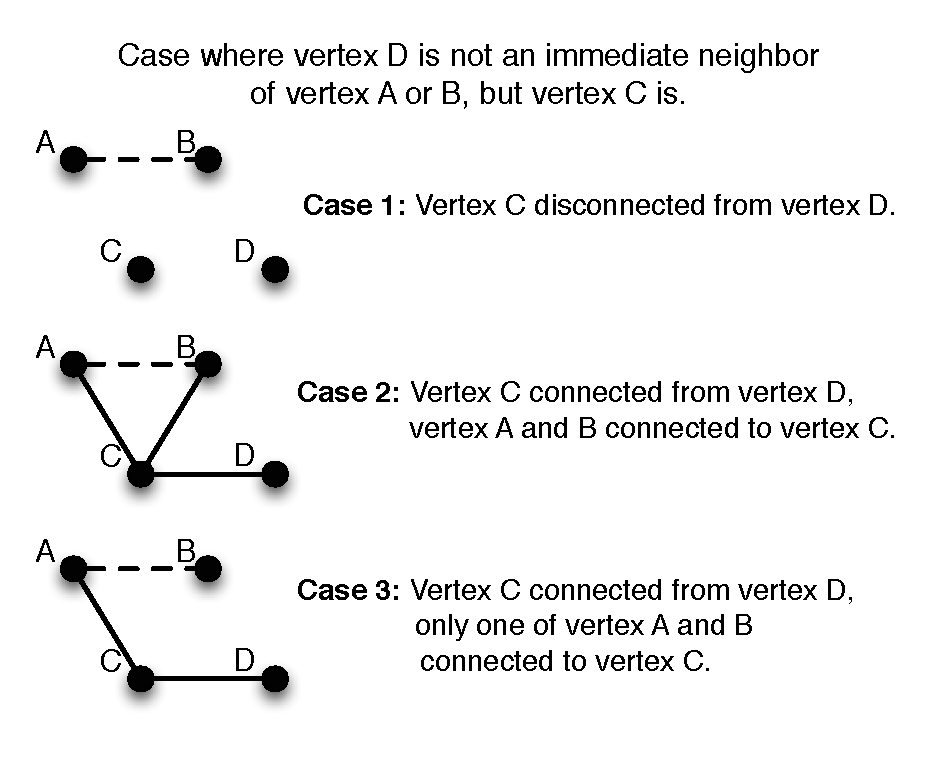
\includegraphics[width=3in]{Figures/case.eps}
\label{fig:case}
\end{figure}

\begin{itemize}
\item Vertex $3$ is not connected to vertex $4$.  In this case, the four vertices can never form a 4-motif, regardless of whether vertices $1$ and $2$ are connected, and we don't have to change the motif counts.
\item Vertex $3$ and $4$ are connected, and vertex $1$ and $2$ are both connected to vertex $3$.  In this case, connecting vertex $1$ and $2$ deletes a four-star motif and adds a triangle-with-edge motif.
\item Vertex $3$ and $4$ are connected, and only one of vertex $1$ and $2$ are connected to vertex $3$.  In this case, connecting vertex $1$ and $2$ creates a four-line motif.
\end{itemize}

It is much faster to test for these cases than to do the normal computations (which would involve finding the induced subgraph on those four vertices, then testing it to see if it was either of the 4-motifs).  So implementing this optimization produces an enormous speedup, allowing us to perform several thousand rewiring steps in one day.

%\begin{algorithm}
%\caption{Our approach}
%\label{algorithm:hillclimbing}
%\begin{algorithmic}
%Initialize graph $G = (V, E)$ with prescribed degree sequence\\
%motifCounts <- CountMotifs($G$)\\
%\Repeat{computation time limit exceeded} {
%	addedMotifCounts <- \{0, \dots, 0\}
%	Choose $e_1, e_2 \in E$ at random\\
%	G_{small} <- InducedSubgraph($G$, secondDegreeNeighbors(e_1.Src, e_1.Dst, e_2.Src, e_2.Dst)\\
%
%	\ForEach{$e = (v_1, v_2)$ \in $(e_1.Src, e_2.Dst)$, $(e_2.Src, e_1.Dst)$}{
%		Add edge $e = (v_1, v_2)$ to graph $G_{small}$\\
%		
%		
%	}
%	Delete edges $(e_1.Src, e_1.Dst)$, $(e_2.Src, e_2.Dst)$\\
%	newMotifCounts <- CountMotifs($G$)\\
%	\eIf {error(newMotifCounts) < error(motifCounts)} {
%		motifCounts <- newMotifCounts\\
%	} {
%		Return graph to original state\\
%	}
%}
%
%\begin{function}
%	\If {edgePresent is True} {
%		Delete edge $(v_1, v_2)$
%	}
%	
%	firstDegreeNeighbors <- GetNeighbors(v_1, v_2)\\
%	secondDegreeNeighbors <- GetNeighbors(firstDegreeNeighbors)\\
%	\Comment{Count 3-motifs}
%	\ForEach{$v_3$ in firstDegreeNeighbors} {
%		\If {$v_1$ and $v_2$ both connected to $v_3$ in $G_{small}$} {
%			mtThreeClosed <- mtThreeClosed + 1
%			mtThreeOpen <- mtThreeOpen - 1
%		} \ElseIf {$v_1$ or $v_2$ are connected to $v_3$ in $G_{small}$} {
%			mtThreeOpen <- mtThreeOpen + 1
%		} \Else {
%			pass
%		}
%	}
%	\Comment{Count 4-motifs}
%	\ForEach{$v_3$ in firstDegreeNeighbors} {
%		\ForEach{$v_4$ in firstDegreeNeighbors} {
%			m = InducedSubgraph($G_{small}$, (v1, v2, v3, v4))
%			\ForEach{motif in ListOfMotifs} {
%				\If{m is instance of motif}
%			}
%		}
%		\ForEach{$v_4$ in secondDegreeNeighbors - firstDegreeNeighbors} {
%		
%		}
%	}
%	\caption{CountAddedMotifs($G_{small}$, $v_1$, $v_2$, bool edgePresent)}
%\end{function}
%
%\end{algorithmic}
%\end{algorithm}